%========================================================================
% Modelo para elaboracao de textos academicos: TCC, dissertacoes e teses
% Elaborado pelo GISIS - Grupo de Imageamento Sismico e Inversao Sismica.
%========================================================================
\chapter{Resultados e Discussões}
\label{ch:resultados}

Neste capítulo, procede-se a apresentação meticulosa dos resultados obtidos por meio da comparação entre os métodos propostos por \citeonline{podvin1991finite}, \citeonline{jeong2008fast} e \citeonline{noble2014accurate}. A análise abarca não apenas a precisão no cálculo dos tempos de trânsito, mas também o desempenho computacional de cada abordagem. Após a exposição desses resultados, empreende-se discussões detalhadas e individualizadas sobre cada método.

No contexto da aplicação no modelo homogêneo, reproduz-se fielmente o experimento conduzido no trabalho de \citeonline{cai2023improved}. Este estudo foi marcado pela introdução de inovações em termos de precisão, notadamente no âmbito do \textit{Fast Iterative Method}. A replicação desse experimento visa proporcionar uma comparação direta com as melhorias propostas por \citeonline{cai2023improved}, estabelecendo um cenário claro para a avaliação do desempenho dos métodos estudados.

Por sua vez, a aplicação no modelo de duas camadas reproduz o experimento minuciosamente detalhado por \citeonline{alves2022refraction}. Este cenário específico foi escolhido para avaliar a robustez e aplicabilidade dos métodos em um contexto que simula condições geofísicas controladas. Além disso, essa abordagem proporciona uma perspectiva de escalabilidade, onde o problema é inicialmente concebido em uma escala reduzida e gradualmente aumenta de tamanho ao longo do estudo, permitindo uma análise do comportamento e eficiência dos métodos à medida que a densidade de células no modelo se intensifica.

A aplicação no modelo complexo expande ainda mais esta análise, destacando o comportamento dos tempos de trânsito em face de expressivos contrastes de velocidade. Este cenário mais desafiador representa um ambiente realista. A análise do tempo de execução para cada método, neste contexto, adiciona uma camada crucial à nossa compreensão, considerando as demandas computacionais em simulações mais representativas. Dessa forma, ao explorar os cenários propostos e considerar os aspectos de desempenho obtidos, evidencia-se uma visão sobre a eficácia dos métodos analisados em diferentes contextos, contribuindo para o avanço do conhecimento na área de modelagem sísmica utilizando a equação eikonal.

\section{Aplicação em modelo homogêneo}

A apresentação detalhada dos resultados obtidos é fornecida na Tabela \ref{table_homog}, na qual são destacados os tempos de execução, o erro médio e o erro máximo associados a cada formulação avaliada. A metodologia adotada para a obtenção desses resultados envolveu a execução da implementação proposta por \citeonline{cai2023improved}, a qual foi conduzida no mesmo ambiente computacional. Esse ambiente foi configurado conforme as diretrizes previamente estabelecidas no capítulo de Metodologia, garantindo consistência e comparabilidade nos experimentos.

A escolha de utilizar a implementação de \citeonline{cai2023improved} decorre da sua disponibilidade pública, o que permite uma análise transparente e passível de replicação por outros pesquisadores. A uniformidade nas configurações de execução, proporciona uma base sólida para a avaliação comparativa das formulações em estudo. Essa abordagem metodológica estruturada não apenas promove a transparência e a reprodutibilidade dos resultados, mas também possibilita uma análise mais aprofundada das características de desempenho de cada formulação. Dessa forma, ao apresentar esses dados de maneira clara e concisa, busca-se contribuir para o entendimento do comportamento dos métodos em um ambiente homogêneo, estabelecendo as bases para interpretações mais refinadas.

\begin{table}[H]
	\caption{Tempo de execução, erro médio e máximo em relação a equação analítica para meio homogêneo. Aplicação dos métodos utilizados relacionando com os resultados do experimento de \citeonline{cai2023improved}.}
	\begin{tabular}{r|ccc}
		\multicolumn{1}{c|}{} & Tempo {[}s{]} & Erro médio {[}s{]} & Erro máximo {[}s{]} \\ \hline
		\citeonline{podvin1991finite} & 0,9661        & 0,000273           & 0,000762    \\ \hline
		\citeonline{jeong2008fast}    & 0,6082        & 0,000837           & 0,001323    \\ \hline
		\citeonline{noble2014accurate}& 0,8085        & 0,000037           & 0,000069    \\ \hline
		\citeonline{cai2023improved}  & 1,9312        & 0,000196           & 0,000282           
	\end{tabular}
	\label{table_homog}
\end{table}

No decorrer do teste no modelo homogêneo, conforme evidenciado na Tabela \ref{table_homog}, é possível discernir a superioridade em desempenho do método proposto por \citeonline{jeong2008fast}. Contudo, é relevante observar que, embora esse método tenha apresentado a melhor performance, os erros registrados revelam-se os mais elevados em comparação com as demais abordagens testadas. O método desenvolvido por \citeonline{cai2023improved}, demonstra a capacidade de atenuar o erro associado ao \textit{Fast Iterative Method}, no entanto, apesar dessa melhoria, não se destaca como o mais preciso entre os métodos analisados, evidenciando, por vezes, uma performance inferior em relação às alternativas examinadas. Dentre as formulações avaliadas, a implementação mais precisa revelou-se aquela do \textit{Fast Sweeping Method}, incorporando a estratégia de paralelização proposta por \citeonline{detrixhe2013parallel} e os operadores desenvolvidos no trabalho de \citeonline{noble2014accurate}. Este método, além de apresentar maior precisão, destaca-se pela eficiência computacional, embora não tenha sido o mais performático isoladamente. No entanto, ao considerar o equilíbrio entre precisão e performance, o \textit{Fast Sweeping Method} revela-se promissor, oferecendo uma alternativa viável e equilibrada para a resolução da equação eikonal em cenários homogêneos. 

O método que evidenciou o mais elevado desempenho computacional foi a forma original do \textit{Fast Iterative Method}, superando em 37\% a formulação proposta por \citeonline{podvin1991finite}, em 24\% considerando o \textit{Fast Sweeping Method} e em expressivos 68\% em relação ao método aprimorado por \citeonline{cai2023improved}. Em instâncias de problemas com dimensões reduzidas, não se observam grandes disparidades nos tempos de execução, ou seja, as diferenças apesar de expressivas, são insignificantes. Nesse contexto, o componente crucial a ser analisado, especialmente em modelos homogêneos, é a precisão. Dentre os métodos avaliados, o \textit{Fast Sweeping Method} se destaca por apresentar a menor discrepância em relação à formulação analítica. Considerando apenas o erro máximo, conforme disposto na Tabela \ref{table_homog}, este método revela reduções significativas de 90\% em comparação com a formulação de \citeonline{podvin1991finite}, 94\% em relação à versão original do \textit{Fast Iterative Method} e 75\% em relação ao \textit{Fast Iterative Method} com operadores precisos. Essa análise apurada não apenas destaca as diferenças de desempenho entre os métodos, mas também ressalta a superioridade do \textit{Fast Sweeping Method} em termos de precisão, consolidando sua posição como uma escolha promissora para aplicações que demandam alta acurácia em modelos homogêneos.

\section{Aplicação em modelo de refração}

A Tabela \ref{table_refModel} oferece uma visão detalhada dos resultados obtidos em um teste de escalabilidade para cada método avaliado. Este teste foi essencial para compreender a capacidade de lidar com o problema em domínios distintos. É importante ressaltar que a análise de reciprocidade desempenha um papel crucial, tornando-se evidente a identificação de possíveis vazamentos de memória quando aplicado múltiplas posições de tiro. Além disso, a validação em aplicações de imageamento sísmico também é contemplada através do estudo de reciprocidade. O tempo de execução assume uma importância crítica na geração eficiente de resultados nessas aplicações. A capacidade dos métodos em manter um desempenho consistente e eficaz, mesmo em cenários de maior exigência computacional, reforça a confiança na sua aplicabilidade prática em contextos mais desafiadores. 

\begin{table}[H]
	\caption{Tempo de execução para cada discretização e reciprocidade para o modelo de 25 m.}
	\begin{tabular}{r|cccc}
		& 100 m    & 50 m     & 25 m     & Reciprocidade \\ \hline
		\citeonline{podvin1991finite}   & 0,0676 s & 0,3141 s & 3,5324 s & 7896,2 s        \\ \hline
		\citeonline{jeong2008fast} & 0,0491 s & 0,0987 s & 0,6261 s & 921,8 s              \\ \hline
		\citeonline{noble2014accurate} & 0,1042 s & 0,2286 s & 0,8284 s & 1382,5 s          \\
	\end{tabular}
	\label{table_refModel}
\end{table}

Os resultados apresentados na Tabela \ref{table_refModel} evidenciam distintos contextos de desempenho. No cenário envolvendo o problema de menor escala, destaca-se a formulação proposta por \citeonline{jeong2008fast}, demonstrando uma vantagem de 27\% e 52\% sobre as formulações de \citeonline{podvin1991finite} e \citeonline{noble2014accurate}, respectivamente. À medida que nos deparamos com o problema de escala intermediária, utilizando a discretização de 50 metros, o \textit{Fast Iterative Method} persiste como o líder em desempenho, apresentando uma superioridade de 68\% e 56\% em relação às formulações de \citeonline{podvin1991finite} e \citeonline{noble2014accurate}, respectivamente. Por fim, no problema de maior densidade de pontos, com a discretização do modelo de 25 metros, a formulação de \citeonline{jeong2008fast} mantém sua posição de destaque, superando em 82\% e 32\% as formulações de \citeonline{podvin1991finite} e \citeonline{noble2014accurate}, respectivamente. Referindo-se ao problema de reciprocidade, após a realização de 1252 disparos com a equação eikonal, observa-se que o \textit{Fast Iterative Method} apresentou o melhor desempenho, evidenciando uma eficiência de 88\% e 33\% em relação às formulações de \citeonline{podvin1991finite} e \citeonline{noble2014accurate}, respectivamente. Vale ressaltar que o estudo de reciprocidade foi conduzido no modelo com espaçamento de 25 metros, o que resultou em métricas percentuais semelhantes entre os estudos de propagação direta e de reciprocidade. Outro ponto relevante a destacar é o melhor desempenho da formulação de \citeonline{noble2014accurate} com o esquema de paralelização proposto por \citeonline{detrixhe2013parallel} em problemas de larga escala em comparação aos demais cenários.

As Figuras \ref{fig:general_refraction_study}, \ref{fig:precision_refraction_study}, e \ref{fig:reciprocity_refraction_study} oferecem uma visão do estudo de precisão, fornecendo detalhes significativos sobre os tempos calculados que percorrem a trajetória desde a fonte até os receptores, tempos diretos, e vice-versa, tempos recíprocos. Cada uma destas figuras destaca informações cruciais sobre o comportamento da solução dos métodos utilizados, representados por cores específicas. O tom azul está associado à formulação proposta por \citeonline{podvin1991finite}, enquanto o amarelo denota a abordagem de \citeonline{jeong2008fast}, e o verde representa a formulação desenvolvida por \citeonline{noble2014accurate}. Além disso, os diferentes estilos de linha desempenham um papel fundamental na comunicação visual, indicando os diversos parâmetros de discretização adotados. Notavelmente, as linhas sólidas representam o modelo com espaçamento de 25 metros, as linhas tracejadas correspondem ao modelo de 50 metros, e as linhas com ponto e traço caracterizam o modelo de 100 metros. Essa diferenciação visual proporciona uma compreensão mais profunda das variações nos resultados, permitindo uma análise mais refinada das influências do parâmetro de discretização nos tempos calculados. 

\begin{figure}[H]
	\centering
	\subfloat[]{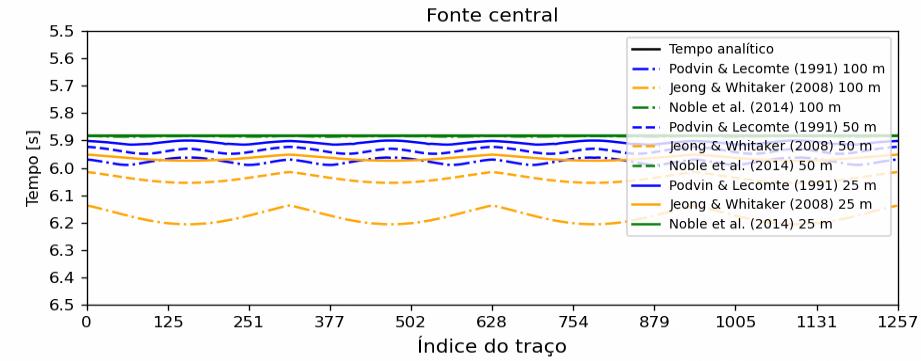
\includegraphics[width=15cm,height=5.4cm]{Imgs/RevisaoBibliografica/precision_direct.png}\label{fig:rnca}}\newline
	\subfloat[]{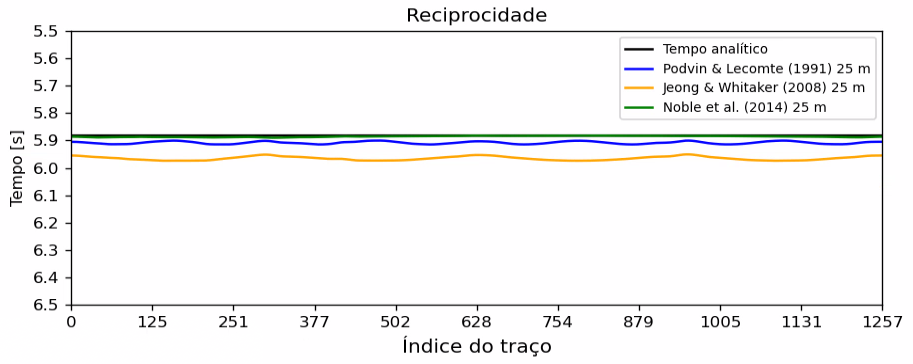
\includegraphics[width=15cm,height=5.4cm]{Imgs/RevisaoBibliografica/reciprocity.png}\label{fig:rncb}} 
	\caption{Panorama geral do comportamento dos tempos de trânsito para todos os métodos estudados. (a) exibe a variação para cada discretização do modelo de velocidade e (b) mostra somente o estudo de reciprocidade aplicado no modelo de 25 m.}
	\label{fig:general_refraction_study}	
\end{figure}

A Figura \ref{fig:general_refraction_study}a) oferece uma visão da configuração de todos os métodos em relação ao tiro central, onde a linha sólida preta representa o tempo analítico associado ao experimento. Essa representação visual permite a comparação direta entre os tempos calculados pelos diferentes métodos e o referencial analítico. Já na Figura \ref{fig:general_refraction_study}b), os tempos registrados são apresentados, utilizando o princípio da reciprocidade, no modelo com discretização de 25 metros. Nesse contexto, é relevante observar que os tempos esperados para esse caso específico se manifestariam como retas horizontais, mantendo-se constantes, dado que o modelo é caracterizado por homogeneidade lateral. Dessa forma, a combinação das informações visuais dessas duas figuras não apenas destaca a configuração geral dos métodos no tiro central, mas também fornece características valiosos sobre a precisão e consistência dos tempos registrados, especialmente quando aplicado o princípio da reciprocidade em um modelo com discretização específica. A configuração sinuosa dos tempos de trânsito é uma característica resultante da solução eikonal implementada em coordenadas cartesianas \cite{white2020pykonal}, em que ângulos de incidência múltiplos de $\pi / 2$ apresentam menores índices de erro.    

\begin{figure}[H]
	\centering
	\subfloat[]{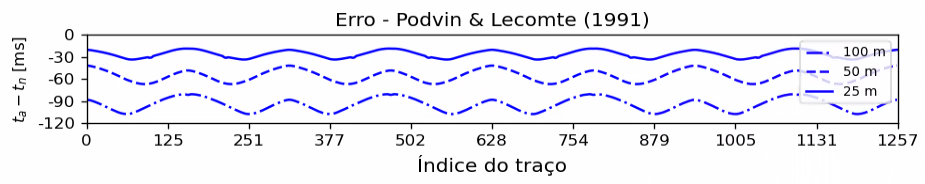
\includegraphics[width=15cm,height=3cm]{Imgs/RevisaoBibliografica/error_pod_direct.png}\label{fig:rncc}}\newline
	\subfloat[]{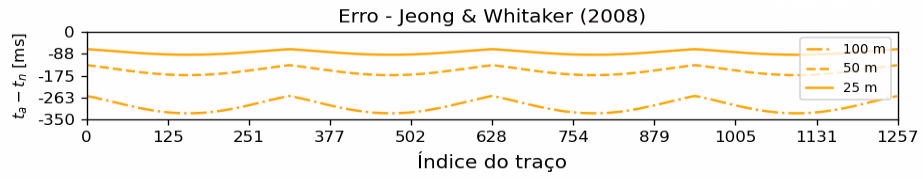
\includegraphics[width=15cm,height=3cm]{Imgs/RevisaoBibliografica/error_fim_direct.png}\label{fig:rnce}}\newline
	\subfloat[]{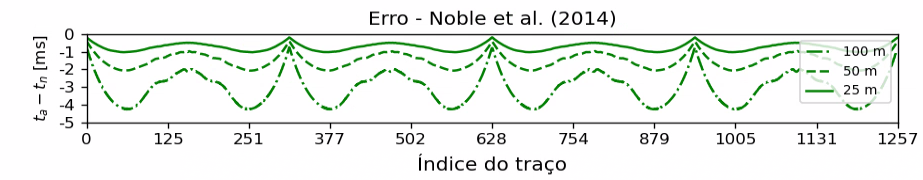
\includegraphics[width=15cm,height=3cm]{Imgs/RevisaoBibliografica/error_fsm_direct.png}\label{fig:rncg}}\newline
		
	\caption{Diferença entre os tempos analítico $t_a$ e numérico $t_n$ por método em relação aos parâmetros de discretização do modelo. (a) o método clássico de \citeonline{podvin1991finite}, (b) o FIM e (c) o FSM utilizando discretizações de 100, 50 e 25 m.}
	\label{fig:precision_refraction_study}	
\end{figure}

A análise visual apresentada na Figura \ref{fig:precision_refraction_study} revela um fenômeno significativo: à medida que a malha de discretização se torna mais esparsa, a discrepância entre a solução analítica e a solução numérica aumenta. Essa observação sugere que os erros associados à solução numérica são proporcionais ao nível de refinamento do modelo, um padrão que emerge das inerentes limitações do método das diferenças finitas. A peculiaridade desse comportamento destaca a sensibilidade do método às características da malha utilizada na discretização do problema. Em outras palavras, a escolha da resolução da malha tem um impacto direto na precisão da solução numérica. Este fenômeno é uma manifestação das limitações intrínsecas do método das diferenças finitas, que, ao lidar com malhas mais esparsas, tende a introduzir erros significativos na estimativa dos tempos de trânsito. Diante dessa constatação, surge a necessidade de estratégias para aprimorar a precisão da solução numérica. Uma abordagem sugerida é a ampliação do operador de diferenças finitas, incorporando mais pontos vizinhos no cálculo dos tempos de trânsito \cite{noble2014accurate, cai2023improved}. Assim o aumento da ordem dos operadores visa mitigar os efeitos negativos da esparsidade da malha, oferecendo uma alternativa para contornar as limitações inerentes e aprimorar a fidelidade da solução numérica.

A Figura \ref{fig:precision_refraction_study}a) ilustra as discrepâncias entre os tempos analítico e numérico em relação à formulação de \citeonline{podvin1991finite}, evidenciando erros máximos para cada discretização de aproximadamente -30, -70 e -110 ms, para malhas de 25, 50 e 100 m, respectivamente. Já a Figura \ref{fig:precision_refraction_study}b) exibe as diferenças em relação à formulação de \citeonline{jeong2008fast}, revelando erros máximos para cada discretização em torno de -90, -170 e -340 ms. Por fim, a Figura \ref{fig:precision_refraction_study}c) apresenta as variações relacionadas à formulação de \citeonline{noble2014accurate}, indicando erros para cada discretização de aproximadamente -1, -2 e -5 ms, para malhas de 25, 50 e 100 m, respectivamente. Ao analisar as informações sobre precisão apresentadas, o \textit{Fast Sweeping Method} destaca-se pela considerável superioridade, produzindo resultados satisfatórios mesmo no cenário de malha esparsa. A abordagem de \citeonline{noble2014accurate}, quando aplicada em larga escala com uma discretização de 25 metros, resultou em um erro inferior a 1 milissegundo, proporcionando uma representação mais fiel do fenômeno cinemático. Em contrapartida, as demais metodologias revelam uma discrepância negativa em relação à equação analítica, indicando um efeito de redução na velocidade do meio, especialmente quando os tempos de trânsito obtidos são maiores que a solução analítica. 

A Figura \ref{fig:reciprocity_refraction_study} evidencia claramente a superioridade em precisão do \textit{Fast Sweeping Method}. No entanto, durante o desenvolvimento do estudo de reciprocidade, a etapa de inicialização gerou instabilidades no processo de modelagem, conforme destacado na Figura \ref{fig:reciprocity_refraction_study}c. Na fase inicial do cálculo dos tempos de trânsito, todo o volume foi inicializado com um valor tendendo ao infinito, enquanto apenas os pontos vizinhos à fonte receberam inicialização com base no tempo analítico para velocidade constante, conforme indicado pela equação \ref{analyticalT}. O procedimento original proposto por \citeonline{noble2014accurate} implementa a inicialização analítica exclusivamente nos pontos do primeiro octante. Contudo, o estudo de reciprocidade revelou a necessidade de estender essa inicialização aos pontos vizinhos em todas as direções, ou seja, nos oito octantes circundantes à fonte, conforme exemplificado na Figura \ref{fig:voxel_full}.

\begin{figure}[H]
	\centering
	\subfloat[]{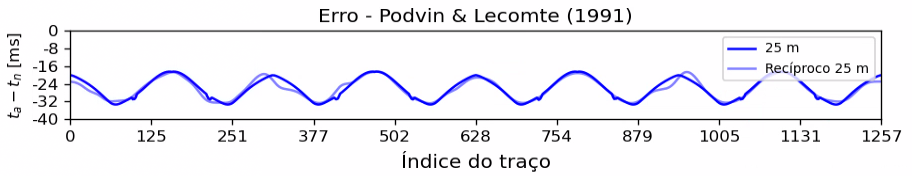
\includegraphics[width=15cm,height=3cm]{Imgs/RevisaoBibliografica/error_pod_reciprocity.png}\label{fig:rncd}}\newline
	\subfloat[]{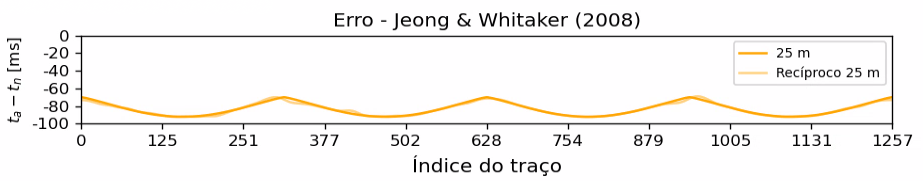
\includegraphics[width=15cm,height=3cm]{Imgs/RevisaoBibliografica/error_fim_reciprocity.png}\label{fig:rncf}}\newline
	\subfloat[]{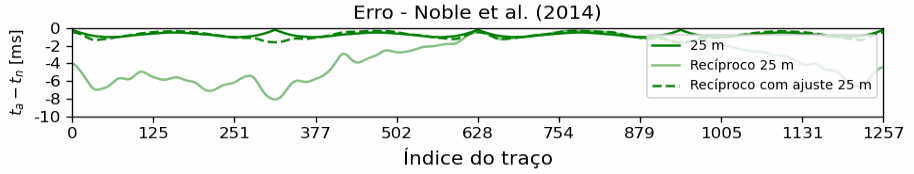
\includegraphics[width=15cm,height=3cm]{Imgs/RevisaoBibliografica/error_fsm_reciprocity.png}\label{fig:rnch}}
	
	\caption{Sobreposição entre os erros dos tempos de trânsito diretos, da fonte para os receptores, e recíprocos, dos receptores para a fonte, em relação à equação analítica. Diferença analítico $t_a$ e numérico $t_n$ em relação aos métodos (a) clássico, (b) FIM e (c) FSM somente para a discretização de 25 m entre os pontos da malha.}  
	\label{fig:reciprocity_refraction_study}
\end{figure}

Após a implementação das correções no algoritmo, procedeu-se a uma nova modelagem utilizando o princípio da reciprocidade, reforçando ainda mais a precisão do \textit{Fast Sweeping Method}, conforme representado pela linha tracejada verde na Figura \ref{fig:reciprocity_refraction_study}c. Cabe destacar que, mesmo diante dessas melhorias, a análise revela alguns erros de interpolação na Figura \ref{fig:reciprocity_refraction_study}. Esses equívocos são atribuíveis à localização dos pontos considerados no círculo de receptores, os quais se encontram fora da malha. Entretanto, é relevante notar que esses erros assumem valores discretos em relação às diferenças entre os tempos analítico e numérico, constituindo um aspecto importante a ser considerado na avaliação da fidedignidade do método.

\section{Aplicação em modelo complexo}

As Figuras \ref{fig:overthrust_inner_circle}, \ref{fig:overthrust_mid_circle} e \ref{fig:overthrust_outer_circle} apresentam os resultados derivados do esquema de modelagem com geometria circular aplicado ao modelo SEG/EAGE \textit{Overthrust}. Novamente, as cores na figura representam cada método, sendo a cor azul atribuída à formulação de \citeonline{podvin1991finite}, o tom laranja a \citeonline{jeong2008fast} e a cor verde à formulação de \citeonline{noble2014accurate}. As figuras consistem em ampliações do sismograma de primeira chegada, com uma seleção específica de estações que destaca a disparidade entre os tempos de trânsito entre as formulações estudadas. Dado que a equação eikonal constitui uma aproximação da equação da onda para altas frequências, é esperado que os detalhes do modelo sejam discerníveis nos dados resultantes. Nesse contexto, as janelas amplificadoras facilitam a identificação desses aspectos.

Conforme delineado no capítulo de metodologia, o esquema de modelagem empregando o modelo complexo inicia-se com três arranjos de receptores circulares, com raios de 5500, 7500 e 9500 metros, espaçados regularmente a cada 25 m, totalizando 5662 estações, para um tiro central na superfície do modelo. Nesse contexto, a Figura 9 apresenta exclusivamente os tempos de trânsito correspondentes às estações 600 até 950 pertencentes ao círculo de raio 5500 m, destacando os pormenores da projeção dos dados no modelo de velocidade. É possível observar que a formulação de \citeonline{jeong2008fast} calcula tempos superiores, enquanto a formulação de \citeonline{podvin1991finite} resulta em tempos intermediários e a formulação de \citeonline{noble2014accurate} alcança tempos inferiores em relação aos métodos numéricos analisados. Os mesmos detalhes podem ser observados nas Figuras \ref{fig:overthrust_mid_circle} e \ref{fig:overthrust_outer_circle}, que correspondem a outras regiões do dado gerado, pertencentes aos círculos com raios de 7500 e 9500 metros, respectivamente.

\begin{figure}[H]
	\centering
	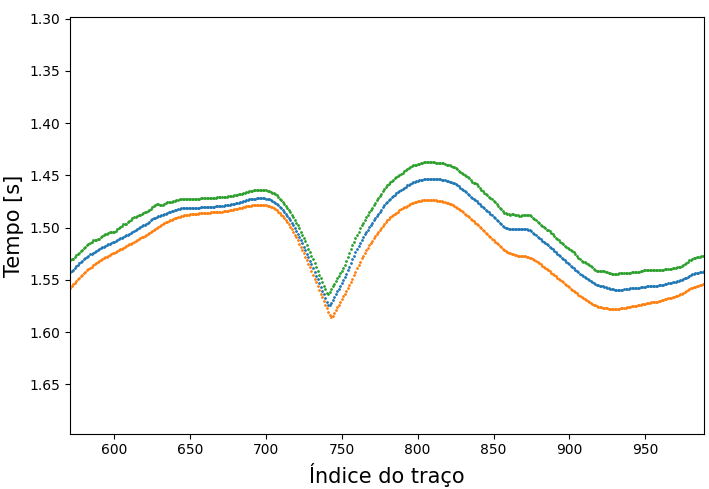
\includegraphics[height=8cm,width=13cm]{Imgs/Resultados/complex_w1.png}		
	\caption{Tempos de trânsito capturados do circulo menor de 5,5 km. As cores representam cada solução numérica, sendo azul para o método clássico, laranja para o FIM e verde para o FSM. O eixo horizontal representa o índice dos receptores entre as 5662 estações e o eixo vertical é o tempo de percurso da frente de onda.}
	\label{fig:overthrust_inner_circle}
\end{figure}

A manifestação intrínseca de atraso nas formulações propostas por \citeonline{podvin1991finite} e \citeonline{jeong2008fast} torna-se evidente ao ser aplicada no contexto do modelo complexo, paralelamente à sua identificação quando utilizada em modelos mais simples. Em contraponto, destaca-se que a formulação elaborada por \citeonline{noble2014accurate} se sobressai ao minimizar os atrasos nos tempos de trânsito, apresentando uma representação mais fiel e precisa do fenômeno cinemático das ondas de primeira chegada.

Com o intuito de enfatizar determinadas regiões que demandam atenção, destaca-se, na Figura \ref{fig:overthrust_inner_circle}, uma faixa compreendida entre os traços 850 e 950, onde se observa um detalhe mais bem representado pela formulação de \citeonline{noble2014accurate}. Enquanto as demais formulações exibem características de tempo de trânsito suavizadas nessa área, o \textit{Fast Sweeping Method} proporciona resultados mais abruptos. Na Figura \ref{fig:overthrust_mid_circle}, entre os traços 1600 e 1650, nota-se que as formulações de \citeonline{podvin1991finite} e \citeonline{noble2014accurate} apresentam semelhanças, porém com atrasos temporais na formulação clássica, ao passo que o \textit{Fast Iterative Method} se revela menos preciso na descrição dos tempos de trânsito. Outro detalhe relevante é evidenciado na Figura \ref{fig:overthrust_outer_circle}, entre os traços 3550 e 3600, onde aspectos mais sutis são melhor representados pela formulação de \citeonline{noble2014accurate}.

\begin{figure}[H]
	\centering
	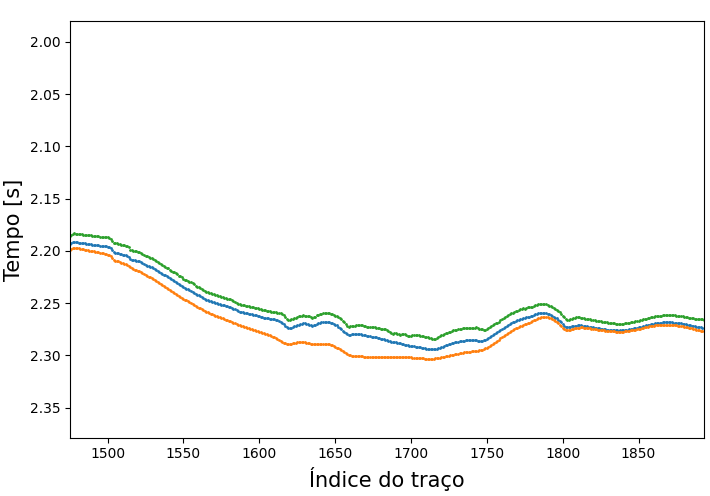
\includegraphics[height=8cm,width=13cm]{Imgs/Resultados/complex_w2.png}	
	\caption{Tempos de trânsito capturados do circulo intermediário de 7,5 km. As cores representam cada solução numérica, sendo azul para o método clássico, laranja para o FIM e verde para o FSM. O eixo horizontal representa o índice dos receptores entre as 5662 estações e o eixo vertical é o tempo de percurso da frente de onda.}
	\label{fig:overthrust_mid_circle}
\end{figure}

\begin{figure}[H]
	\centering
	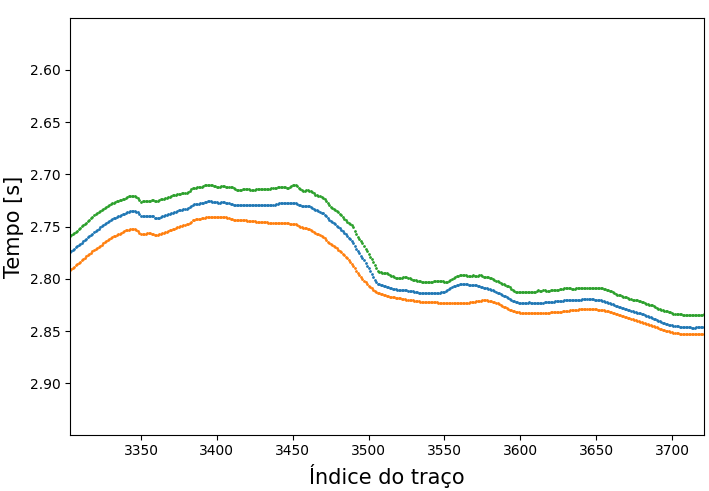
\includegraphics[height=8cm,width=13cm]{Imgs/Resultados/complex_w3.png} \newline 
	
	\caption{Tempos de trânsito capturados do círculo maior de 9,5 km. As cores representam cada solução numérica, sendo azul para o método clássico, laranja para o FIM e verde para o FSM. O eixo horizontal representa o índice dos receptores entre as 5662 estações e o eixo vertical é o tempo de percurso da frente de onda.}
	\label{fig:overthrust_outer_circle}
\end{figure}

A Tabela \ref{table_overthrust} expõe os tempos de execução correspondentes a cada método ao considerar o modelo complexo com geometria circular, utilizando apenas um tiro no centro do modelo. A superioridade em desempenho computacional é creditada ao método de \citeonline{jeong2008fast}, no entanto, essa abordagem apresenta atrasos significativos em relação aos tempos de trânsito calculados, quando comparada à equação analítica e aos demais métodos avaliados. Ao relacionar métricas de eficiência computacional, observa-se que a formulação proposta por \citeonline{podvin1991finite} apresentou um desempenho 78\% inferior, enquanto o \textit{Fast Sweeping Method}, implementado com a paralelização de \citeonline{detrixhe2013parallel}, demonstrou um desempenho de 26\% abaixo da formulação mais eficiente. Portanto, ao considerar a precisão que o \textit{Fast Sweeping Method} pode proporcionar, a sua aplicação em problemas de larga escala se revela vantajosa.

\begin{table}[H]
	\caption{Tempo de execução para a aplicação dos métodos no modelo complexo.}
	\begin{tabular}{r|c}
		& Tempo de execução \\ \hline
		\citeonline{podvin1991finite} & 11,7128 s  \\ \hline
		\citeonline{jeong2008fast} & 2,5595 s      \\ \hline
		\citeonline{noble2014accurate} & 3,4746 s         
	\end{tabular}
	\label{table_overthrust}
\end{table}

No contexto do modelo homogêneo, evidenciou-se a destacada performance do método proposto por \citeonline{jeong2008fast}, embora esse tenha registrado maiores margens de erro em comparação com as demais formulações. A tentativa de aprimoramento do \textit{Fast Iterative Method} conduzida por \citeonline{cai2023improved}, embora tenha contribuído para a redução de erros, não se sobressaiu como a abordagem mais precisa.  O \textit{Fast Sweeping Method}, notadamente quando aplicado com a estratégia de paralelização sugerida por \citeonline{detrixhe2013parallel}, emergiu como uma alternativa que equilibra eficiência computacional e precisão. A análise de reciprocidade, lançou luz sobre questões relativas à inicialização dos métodos e confiabilidade na interpolação em pontos fora da malha. A correção aplicada ao \textit{Fast Sweeping Method} para abranger inicializações em todas as direções, conforme indicado pelo estudo de reciprocidade, fortaleceu ainda mais sua reputação como uma escolha robusta. No cenário utilizando a complexidade do modelo \textit{Overthrust}, os dados gerados proporcionaram uma compreensão vívida das diferenças nos tempos de trânsito calculados por cada método. A performance e a precisão são fatores determinantes, e a decisão de qual método numérico utilizar deve ser orientada pelas necessidades particulares de cada cenário, considerando tanto os requisitos de eficiência computacional quanto a busca por resultados precisos. Portanto, a superioridade do \textit{Fast Sweeping Method} em representar detalhes alinhados à realidade reforçaram sua posição como uma opção versátil e precisa. 




